\documentclass[12pt]{article}
\usepackage[T2A]{fontenc}
\usepackage[utf8]{inputenc}
\usepackage[english,russian]{babel}
\usepackage{a4wide}
\usepackage{float}
\usepackage{graphicx}
\usepackage{amssymb}
\usepackage{amsmath}
\usepackage{color}
\usepackage{url}
\usepackage{tikz}
\usetikzlibrary{matrix}

\usepackage[numbers,sort&compress]{natbib}

\DeclareMathOperator*{\argmax}{arg\,max}
\DeclareMathOperator*{\argmin}{arg\,min}
\newcommand*{\No}{No.}

\usepackage[pdftex,unicode, 
colorlinks=true,
linkcolor = blue
]{hyperref}	% нумерование страниц, ссылки!!!!ИМЕННО В ТАКОМ ПОРЯДКЕ СО СЛЕДУЮЩИМ ПАКЕТОМ
\newcommand{\hdir}{.}

\newcommand{\bx}{\mathbf{x}}
\newcommand{\by}{\mathbf{y}}
\newcommand{\bw}{\mathbf{w}}
\newcommand{\ba}{\mathbf{a}}
\newcommand{\bz}{\mathbf{z}}
\newcommand{\bb}{\mathbf{b}}
\newcommand{\bY}{\mathbf{Y}}
\newcommand{\bX}{\mathbf{X}}
\newcommand{\bu}{\mathbf{u}}
\newcommand{\bt}{\mathbf{t}}
\newcommand{\bp}{\mathbf{p}}
\newcommand{\bq}{\mathbf{q}}
\newcommand{\bc}{\mathbf{c}}
\newcommand{\bP}{\mathbf{P}}
\newcommand{\bT}{\mathbf{T}}
\newcommand{\bB}{\mathbf{B}}
\newcommand{\bQ}{\mathbf{Q}}
\newcommand{\bC}{\mathbf{C}}
\newcommand{\bE}{\mathbf{E}}
\newcommand{\bF}{\mathbf{F}}
\newcommand{\bU}{\mathbf{U}}
\newcommand{\bW}{\mathbf{W}}

% greek bold lower
\newcommand{\bepsilon}{\boldsymbol{\varepsilon}}
\newcommand{\btheta}{\boldsymbol{\theta}} 
\newcommand{\blambda}{\boldsymbol{\lambda}} 
\newcommand{\bchi}{\boldsymbol{\chi}}
\newcommand{\bnu}{\boldsymbol{\nu}}
\newcommand{\bpi}{\boldsymbol{\pi}} 
\newcommand{\bmu}{\boldsymbol{\mu}} 
\newcommand{\btau}{\boldsymbol{\tau}}
\newcommand{\bsigma}{\boldsymbol{\sigma}} 
\newcommand{\bupsilon}{\boldsymbol{\upsilon}}
\newcommand{\bphi}{\boldsymbol{\phi}} 
\newcommand{\bpsi}{\boldsymbol{\psi}} 

\newcommand{\T}{^{\text{\tiny\sffamily\upshape\mdseries T}}}

\usepackage{graphicx}

\graphicspath{{../figures/}}
\newtheorem{definition}{Определение}[section]

\usepackage{subcaption}
\usepackage{neuralnetwork}


\begin{document}
	\title{Симметрия моделей нейронных сетей в задаче моделирования динамики физических систем\thanks{no}}
	\date{}
	\author{}
	\maketitle
	
	\begin{center}
		\bf
		П.\,А.~Северилов\footnote{Московский физико-технический институт, severilov.pa@phystech.edu}, 
		В.\,В.~Стрижов\footnote{Вычислительный центр имени А.\,А.\,Дородницына Федерального исследовательского центра <<Информатика и управление>> Российской академии наук, Московский физико-технический институт, strijov@phystech.edu}
	\end{center}
	{\begin{quote}
			\textbf{Аннотация:}
			Лагранжевы нейронные сети (LNN) были разработаны для получения динамики ограниченного набора физических систем, что делает этот подход относительно узким. В данной работе рассматривается в терминах симметрий теорем Нётер связь моделей LNN с нейронными сетями более общего назначения с долговременной кратковременной памятью (LSTM), которая отлично подходит для прогнозирования последовательных задач, с базовой полносвязной модели нейронной сети (FC) и моделью Neural ODE, разработанной для решения дифференциальных уравнений. Эксперименты сравнения проводились на задаче моделирования физической системы двойного маятника. 
			
			\smallskip
			\textbf{Ключевые слова}: 
			\smallskip
			
			%\textbf{DOI}: 00.00000/00000000000000
		\end{quote}
	}

	
	\section{Введение}
	
	
	%\section{Подходы получения динамики физической системы}
	В классической механике, чтобы получить динамику физической системы, необходимо расписать все силы системы, уравнения сохранения импульса и энергии. Однако на практике моделирование динамики систем данным способом представляется затруднительным. Например, для системы двойного маятника.
	
	Альтернативным подходом является лагранжева динамика, которая переформулирует  проблему в терминах набора обобщенных координат, которые полностью описывают возможные движения частицы. Чтобы использовать лагранжеву динамику, необходимо построить лагранжиан $L$, который определяется как разница между кинетической энергией ($T$) и потенциальной энергией ($U$) системы:
	$$L = T - U $$
	
	Интеграл $L$ по времени называется \textit{действием}. Истинная траектория системы минимизирует этот интеграл (\textit{принцип наименьшего действия}). Отсюда следует, что действие не может меняться при малых вариациях пути, что эквивалентно уравнению Эйлера-Лагранжа
	$$
	\frac{\partial L}{\partial x}-\frac{d}{d t} \frac{\partial L}{\partial \dot{x}}=0
	$$
	
	Теорема Нетер говорит о том, что любая непрерывная симметрия $L$ связана с сохраняющейся величиной системы. Например, если $L$ не меняется при трансляции (т. е. обладает трансляционной симметрией), то сохраняется импульс. Если $L$ не меняется при сдвигах во времени, то сохраняется энергия.
	
	Получение динамики физической системы с помощью нейронных сетей обычно не учитывают законы сохранения и симметрию Нетер \cite{NEURIPS2019_26cd8eca, NEURIPS2019_26cd8eca, NEURIPS2019_26cd8eca}. Простейшие подходы предсказывают ускорение, получая на вход координаты и скорости системы. Лагранжевы нейронные сети (LNN) используют альтернативный метод: предсказывается лагранжиан системы, из него дифференцированием получают динамику системы. Уравнение Эйлера-Лагранжа сохраняют энергию с течением времени, поэтому эта симметрия встроена в нейронную сеть LNN.
	
	\section{Связанные работы}
	%\subsection{Physics informed neural networks}
	%\subsection{HNN}
	%Модель гамильновой нейронной сети \cite{NEURIPS2019_26cd8eca}
	
	
	\section{Лагранжевы нейронные сети}
	\subsection{Лагранжева механика}
	\begin{itemize}
		\item \textbf{Проблемы HNN}: гамильтонов формализм требует, чтобы координаты системы были «каноническими»($(\textbf{q, p})$ должны подчиняться соотношениям, заданным скобками Пуассона) %-- многие системы не удовлетворяют этому ограничению (часто $p \neq q \cdot m$)
		\item \textbf{Решение проблемы}: использовать лагранжианы систем (обеспечивают сохранение полной энергии, могут делать это с использованием произвольных координат)
	\end{itemize}
	
	\textbf{Моделирование динамики системы с помощью лагранжиана}
		\begin{enumerate}
			\item Найти аналитические выражения для кинетической и потенциальной энергии $(T, V )$
			\item Записать лагранжиан $\mathcal{L} = T - V $
			\item Применить ограничение Эйлера-Лагранжа $\frac{d}{d t} \frac{\partial \mathcal{L}}{\partial \dot{q}_{j}} =\frac{\partial \mathcal{L}}{\partial q_{j}} $
			\item Решить получившуюся систему дифференциальных уравнений
		\end{enumerate}

	
	\subsection{Лагранжевы нейронные сети}
	

	
	\subsection{DeLaN}
	Работа, в котором авторы рассматривают моделирование определенных типов лагранжевых систем. Предполагается, что кинетическая энергия является $T = \dot{q}^TM\dot{q}$, где M — q-зависимая положительно определенная матрица. 
	
	Этот подход хорошо работает для динамики твердого тела, которая включает в себя множество систем, встречающихся в робототехнике. Однако многие системы не обладают такой кинетической энергией: заряженная частица в магнитном поле, быстро движущийся объект в СТО.
	
	\subsection{LNN}
	Лагранжевы нейронные сети(LNN)
	Ключевой идеей является параметризовать нейронной сетью лагранжиан $\mathcal{L}$, получить выражение ограничения Эйлера-Лагранжа, обратно распространить ошибку через полученные ограничения.
	
	Получение динамики системы из предсказанного лагранжиана	
	$$
		\begin{aligned}
		\frac{d}{d t} \frac{\partial \mathcal{L}}{\partial \dot{q}_{j}} =\frac{\partial \mathcal{L}}{\partial q_{j}}  \Rightarrow \frac{d}{d t} \nabla_{\dot{q}} \mathcal{L} =\nabla_{q} \mathcal{L} \\
		\left(\nabla_{\dot{q}} \nabla_{\dot{q}}^{\top} \mathcal{L}\right) \ddot{q}+\left(\nabla_{q} \nabla_{\dot{q}}^{\top} \mathcal{L}\right) \dot{q} =\nabla_{q} \mathcal{L} \\
		\ddot{q} =\left(\nabla_{\dot{q}} \nabla_{\dot{q}}^{\top} \mathcal{L}\right)^{-1}\left[\nabla_{q} \mathcal{L}-\left(\nabla_{q} \nabla_{\dot{q}}^{\top} \mathcal{L}\right) \dot{q}\right]
		\end{aligned}
		$$
	
	Таким образом, для заданного набора координат $x_t = (q_t, \dot{q}_t)$ получили метод вычисления $\dot{x}_t = (\dot{q}_t, \ddot{q}_t)$ из параметризованного лагранжиана.
	 
	 Исходя из вышесказанного получаем \textbf{функцию ошибки}: $$\mathcal{L} = \left\|\dot{x}^{\mathcal{L_{\theta}}}_t -\dot{x}^{true}_t\right\|_{2}$$

	\begin{figure}[H]
		\centering
		\begin{subfigure}[b]{0.49\textwidth}
			\centering
			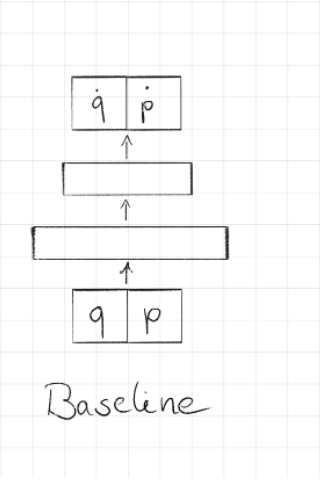
\includegraphics[width=0.6\textwidth]{baseline_nn_scheme.png}
			\caption{Схема работы базового решения моделирования динамики физической системы нейронными сетями}
			\label{fig:y equals x}
		\end{subfigure}
		\hfill
		\begin{subfigure}[b]{0.49\textwidth}
			\centering
			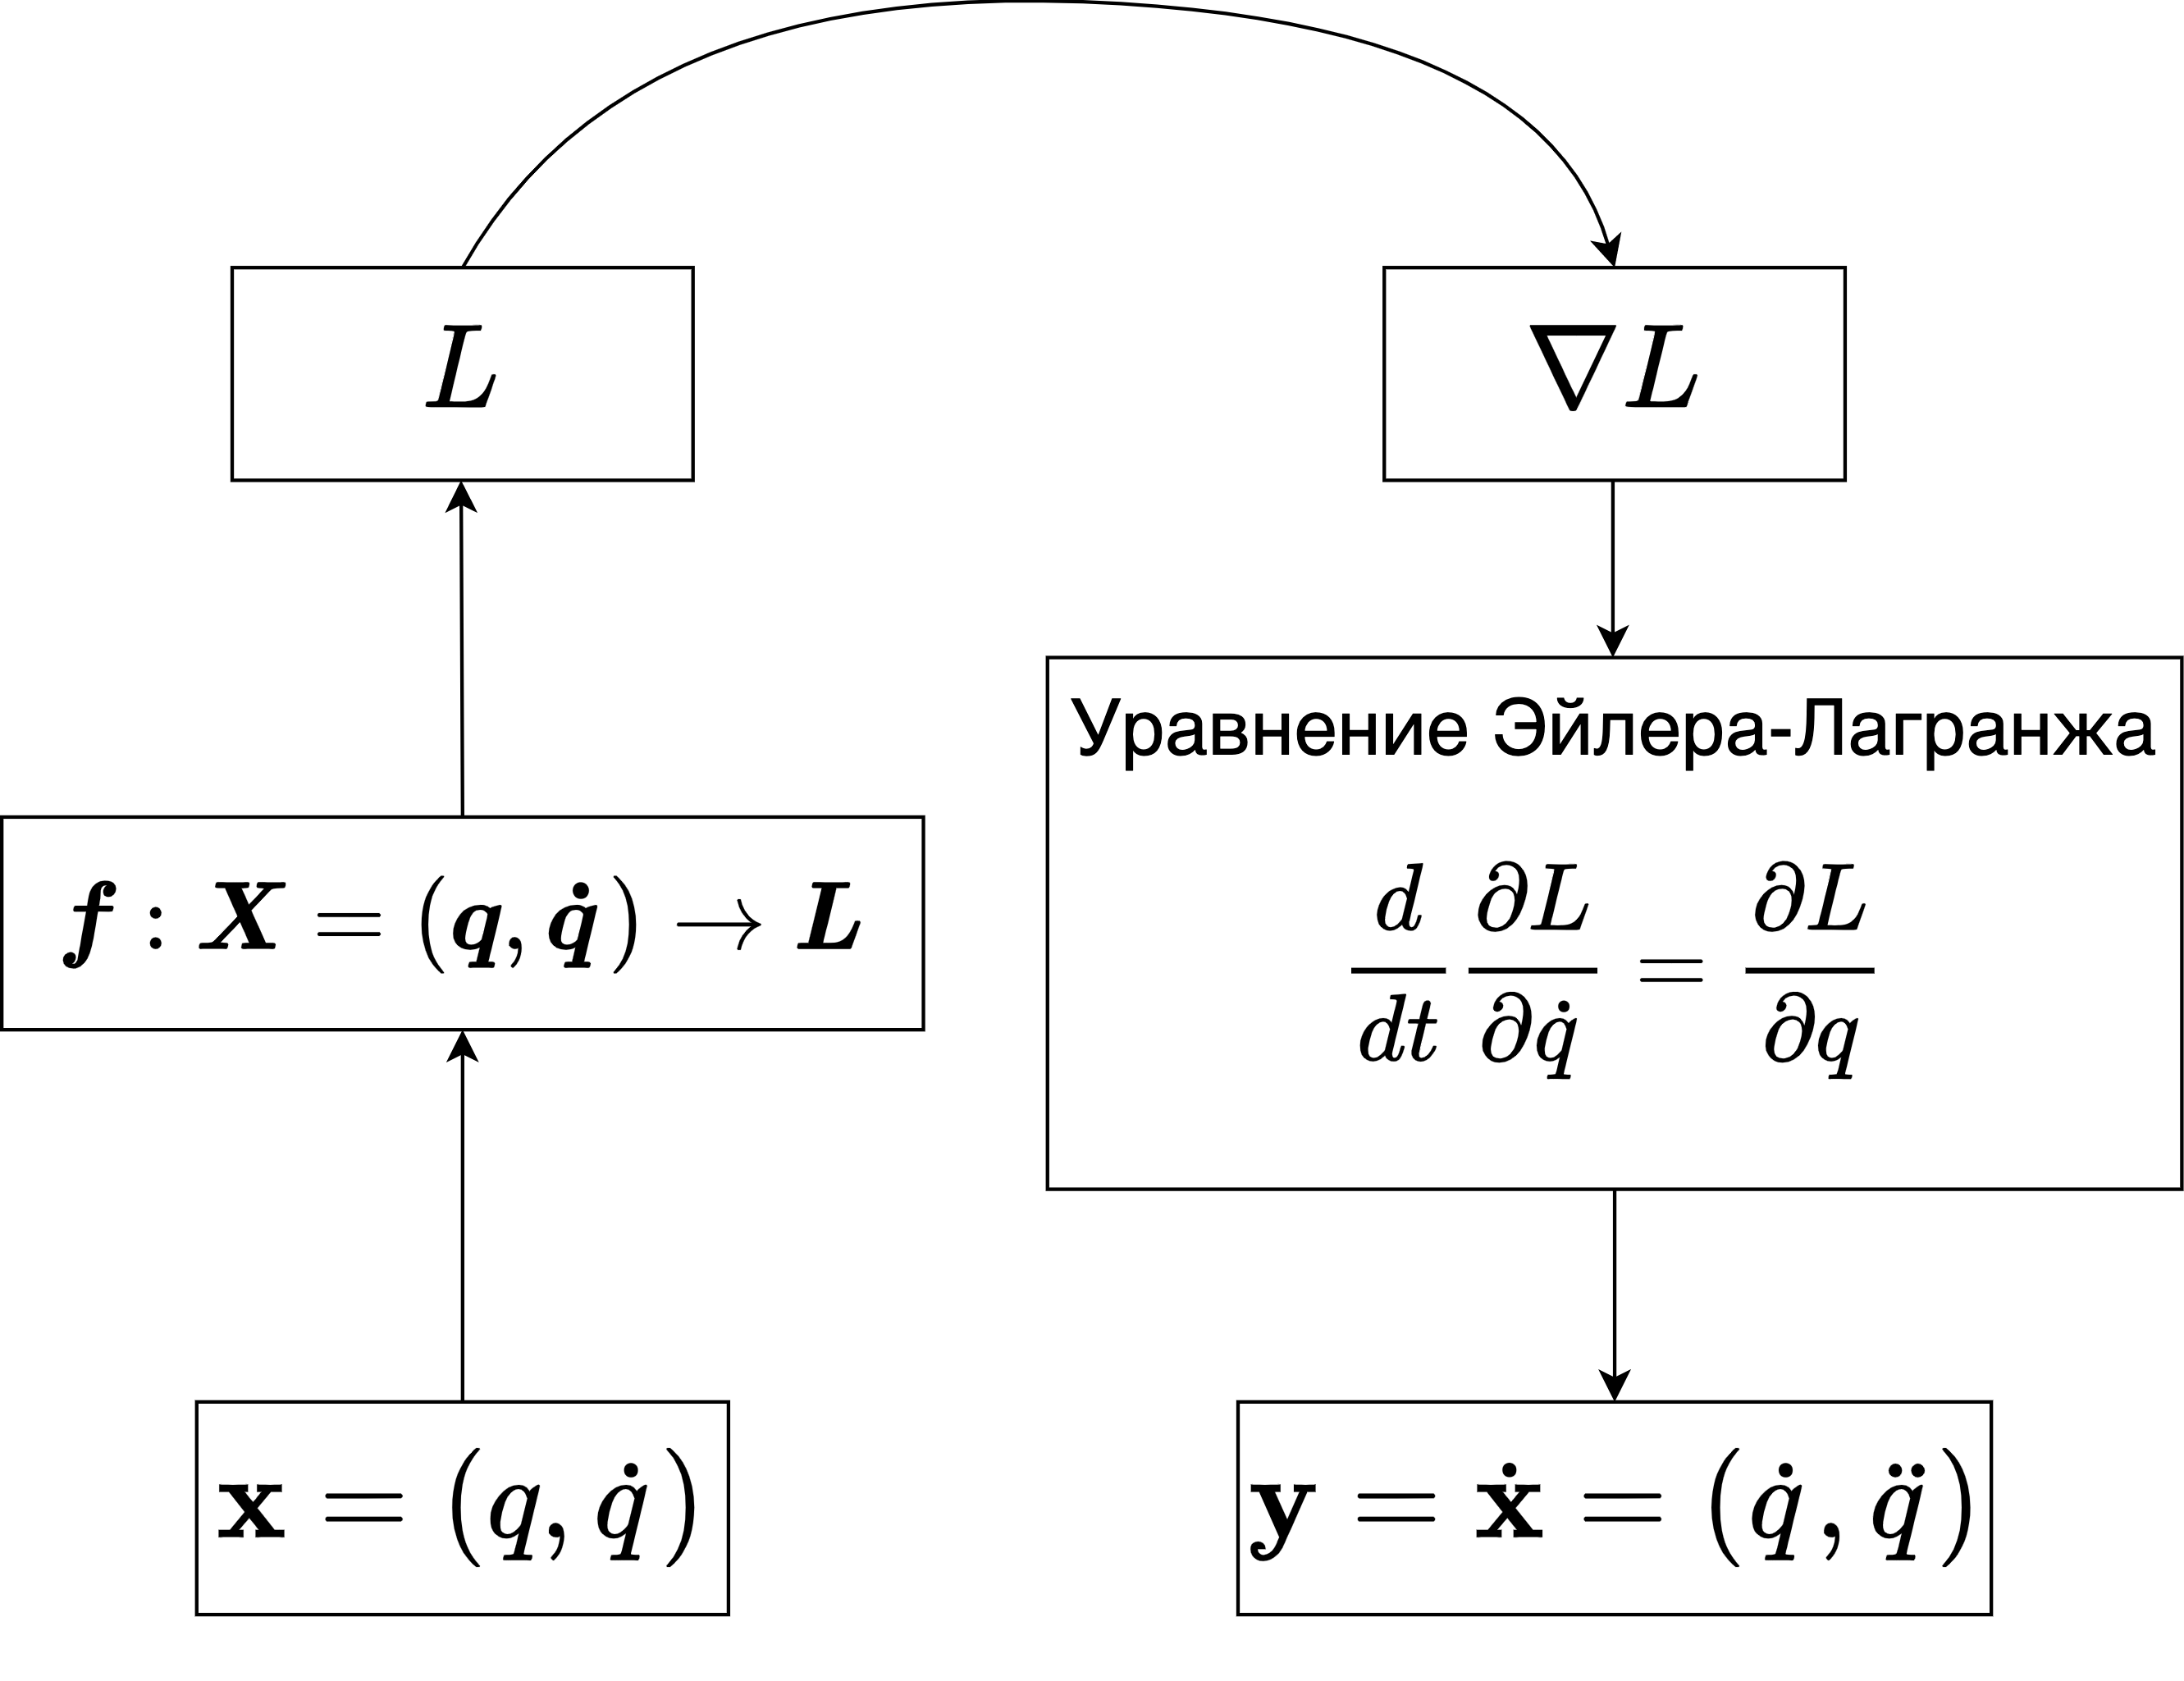
\includegraphics[width=\textwidth]{lnn_scheme.png}
			\caption{Схема работы Lagrangian Neural Networks (LNN) моделирования динамики физической системы}
			\label{fig:three sin x}
		\end{subfigure}
	\end{figure}

	
	\section{Теорема Нётер}
	\textbf{Определение 1 (Генераторы и инвариантность)}. Пусть $L(t, x,\dot{x})$ -- лагранжиан. Рассматривается преобразование 
	\begin{equation}
	\begin{aligned}
	t \mapsto t^{\prime} &=T(t, \boldsymbol{x}, \epsilon) \\
	\boldsymbol{x} \mapsto \boldsymbol{x}^{\prime} &=X(t, \boldsymbol{x}, \epsilon)
	\end{aligned}
	\end{equation}
	где преобразование является гладким как функция от $\epsilon$ и при $\epsilon= 0$ является тождественным и. Пусть
	\begin{equation}
	\begin{array}{l}
	T(t, \boldsymbol{x}, \epsilon)=t+\tau(t, \boldsymbol{x}) \epsilon+O\left(\epsilon^{2}\right) \\
	X(t, \boldsymbol{x}, \epsilon)=\boldsymbol{x}+\xi(t, \boldsymbol{x}) \epsilon+O\left(\epsilon^{2}\right)
	\end{array}
	\end{equation}
	Члены $\tau (t, x)$ и $\xi (t, x)$ называются генераторами преобразования. Генератор оставляет Лагранжиан инвариантным, если
	\begin{equation}
	\mathcal{L}\left(t^{\prime}, \boldsymbol{x}^{\prime}, \dot{x}^{\prime}\right) \frac{d t^{\prime}}{d t}-\mathcal{L}(t, \boldsymbol{x}, \dot{\boldsymbol{x}})=O\left(\epsilon^{2}\right)
	\end{equation}
	
	\textbf{Теорема 1 (Закон сохранения Нётер)}.
	Пусть $\mathcal{L}(t, \boldsymbol{x}, \dot{\boldsymbol{x}})$ -- лагранжиан, инвариантный относительно генераторов $\tau(t, \boldsymbol{x})$ и $\boldsymbol{\xi}(t, \boldsymbol{x})$. Пусть $\boldsymbol{x}(t)$ -- экстремальная функция $J[\boldsymbol{x}]=\int \mathcal{L}(t, \boldsymbol{x}, \dot{\boldsymbol{x}}) d t$. Тогда
	$$
	\left\langle\frac{\partial \mathcal{L}}{\partial \dot{x}}, \boldsymbol{\xi}\right\rangle+\left(\mathcal{L}-\left\langle\dot{\boldsymbol{x}}, \frac{\partial \mathcal{L}}{\partial \dot{\boldsymbol{x}}}\right\rangle\right) \tau
	$$
	сохраняется по $\boldsymbol{x}(t)$.
	%\textbf{Сравнение}
	%	\begin{figure}[h]
	%		\centering
	%		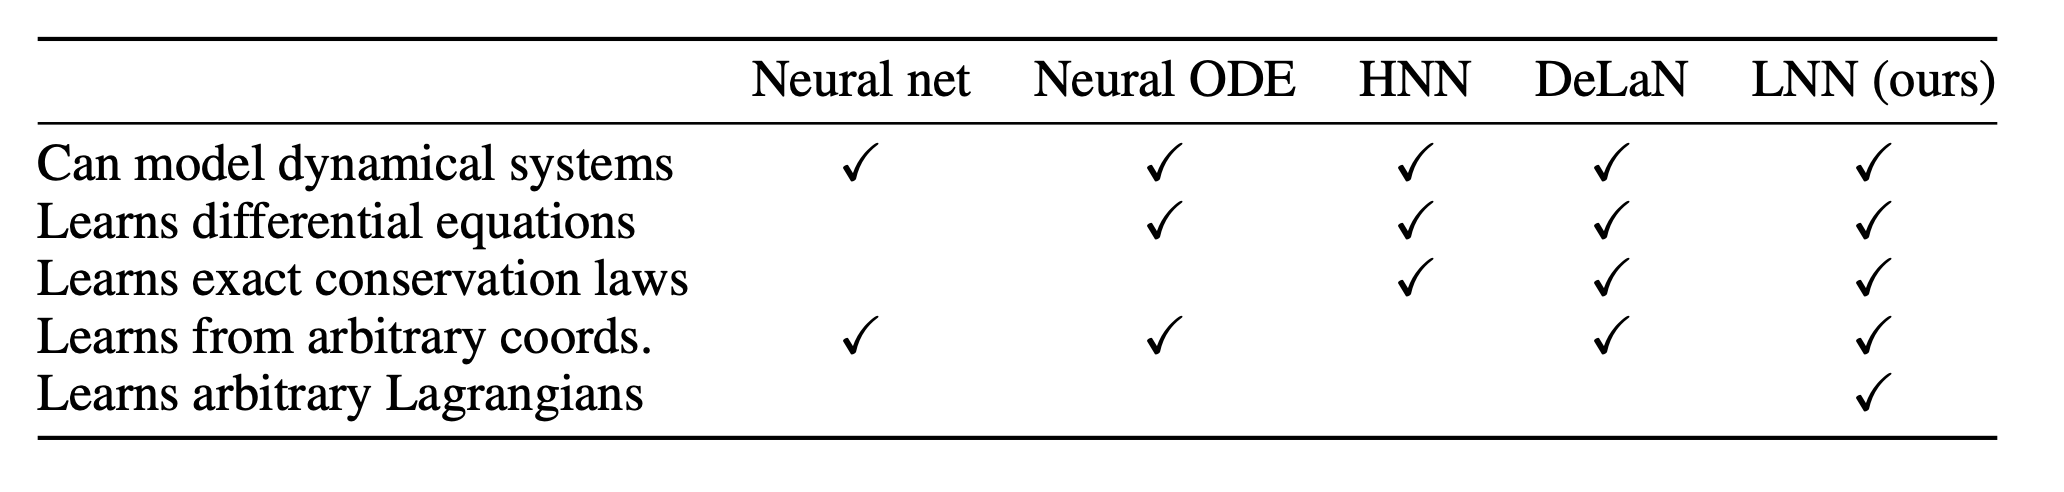
\includegraphics[width=1.05\textwidth]{comparison.png}
	%		\caption{Сравнение подходов моделирования физических систем нейронными сетями}
	%	\end{figure}
	
	
	%\subsection{Сверточные лагранжевы нейронные сети}
	%Добавление сверточных слоев в LNN/DeLaN
	
	\section{Вычислительный эксперимент}
	В рамках вычислительного эксперимента написан программный комплекс для решения поставленных задач~\cite{source_code}.
	
	\subsection{Постановка задачи}
	
	Пусть дана выборка $(\bX, \bY)$, где $\textbf{X} = [\textbf{x}_1, \dots, \textbf{x}_{n}]^{\T} \in \mathbb{R}^{n \times m}$~--- матрица независимых переменных, $\textbf{Y} = [\textbf{y}_1, \dots, \textbf{y}_n]^{\T} \in \mathbb{R}^{n \times k}$~--- матрица целевых переменных.
	
	\subsection{Данные}
	
	В качестве моделируемой физической системы взята система двойного маятника (Рис. \ref{fig:pendulum_system}). Двойной маятник образуется путем присоединения одного маятника к другому. Каждый маятник состоит из груза, соединенного с безмассовым жестким стержнем, который может двигаться только в вертикальной плоскости. Ось первого маятника закреплена в точке $O$. Все движения без трения.
	
	Данная система имеет лагранжиан:
	$$
	\begin{aligned}
	L=\frac{1}{2}\left(m_{1}+m_{2}\right) l_{1}^{2} \dot{\theta}_{1}^{2} &+\frac{1}{2} m_{2} l_{2}^{2} \dot{\theta}_{2}^{2}+m_{2} l_{1} l_{2} \dot{\theta}_{1} \dot{\theta}_{2} \cos \left(\theta_{1}-\theta_{2}\right) \\
	&+\left(m_{1}+m_{2}\right) g l_{1} \cos \theta_{1}+m_{2} g l_{2} \cos \theta_{2}
	\end{aligned}
	$$
	
	\begin{figure}[H]
		\centering
		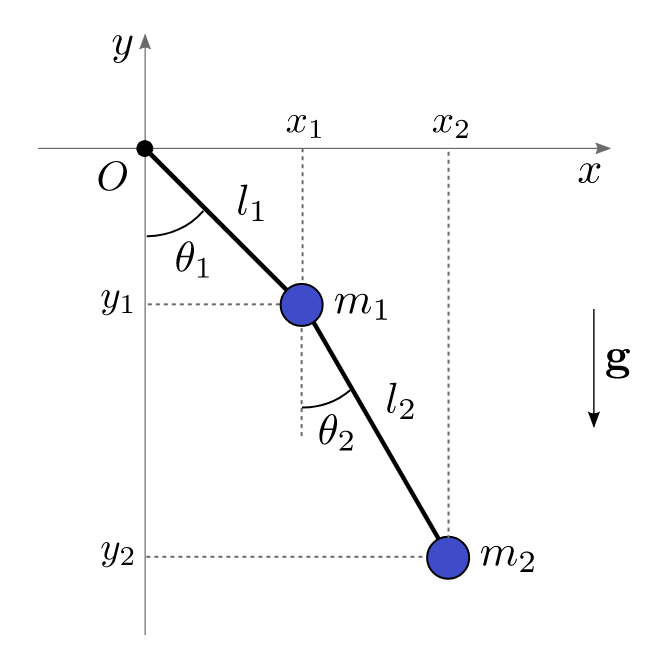
\includegraphics[width=0.4\textwidth]{double_pendulum_scheme.png}
		\caption{Cхема физической системы двойного маятника}
		\label{fig:pendulum_system}
	\end{figure}

	Исходя из данного лагранжиана получаем канонические координаты системы (Рис. \ref{fig:canon})
	\begin{equation}
	\begin{array}{l}
	p_{\theta_{1}}=\frac{\partial L}{\partial \dot{\theta}_{1}}=\left(m_{1}+m_{2}\right) l_{1}^{2} \dot{\theta}_{1}+m_{2} l_{1} l_{2} \dot{\theta}_{2} \cos \left(\theta_{1}-\theta_{2}\right) \\
	p_{\theta_{2}}=\frac{\partial L}{\partial \dot{\theta}_{2}}=m_{2} l_{2}^{2} \dot{\theta}_{2}+m_{2} l_{1} l_{2} \dot{\theta}_{1} \cos \left(\theta_{1}-\theta_{2}\right)
	\end{array}
	\end{equation}


	\begin{figure}[H]
		\centering
		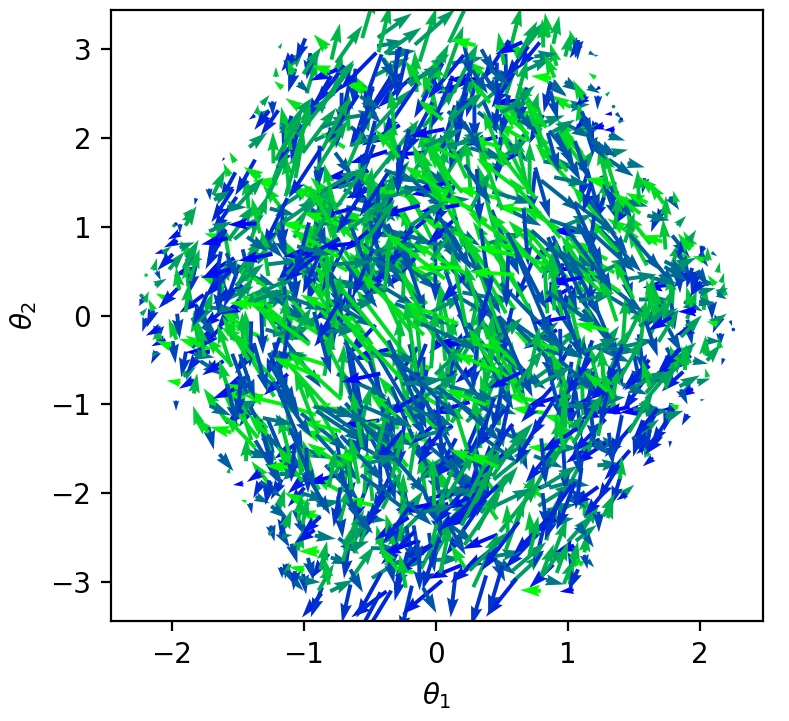
\includegraphics[width=0.9\textwidth]{train_test_data_vis.png}
		\caption{Визуализация данных канонических координат системы двойного маятника}
		\label{fig:canon}
	\end{figure}
	
	\subsection{Исследуемые модели нейронных сетей}
	\subsubsection{Полносвязная нейронная сеть}
	\begin{equation}
	f_{\boldsymbol{w}}(\boldsymbol{x}):=\sigma_{K}\left(W^{(K)} \sigma_{K-1}\left(W^{(K-1)} \cdots \sigma_{1}\left(W^{(1)} \boldsymbol{x}\right)\right)\right)
	\end{equation}
	
	\subsubsection{LSTM}
	\subsubsection{Neural ODE}
	\subsubsection{LNN}
	
	\subsection{Результаты}
	Результаты моделирования динамики системы двойного маятника различными видами нейронных сетей представлены на рисунке \ref{fig:three graphs}
	
	\begin{figure}[H]
		\centering
		\begin{subfigure}[b]{0.49\textwidth}
			\centering
			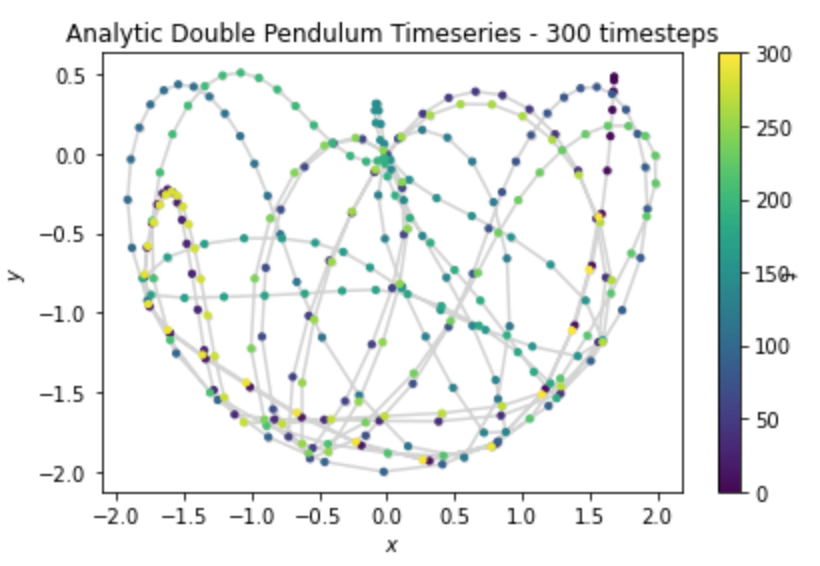
\includegraphics[width=\textwidth]{analytical_pendulum.png}
			\caption{Аналитическое решение}
			\label{fig:y equals x}
		\end{subfigure}
		\hfill
		\begin{subfigure}[b]{0.49\textwidth}
			\centering
			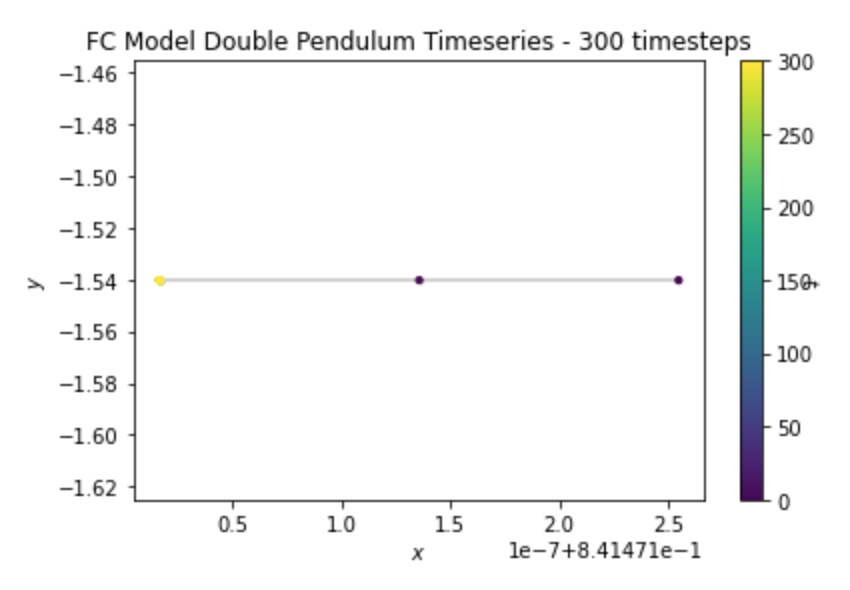
\includegraphics[width=\textwidth]{fc_pendulum.png}
			\caption{Динамика системы с помощью полносвязной нейронной сети}
			\label{fig:three sin x}
		\end{subfigure}
				\hfill
				\vfill
		\begin{subfigure}[b]{0.49\textwidth}
			\centering
			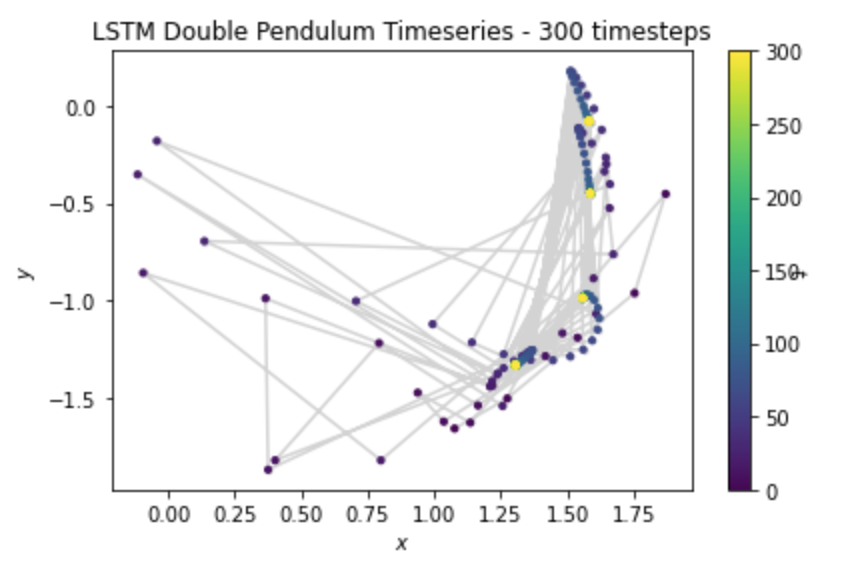
\includegraphics[width=\textwidth]{lstm_pendulum.png}
			\caption{Динамика системы с помощью LSTM}
			\label{fig:three sin x}
		\end{subfigure}
			\hfill
		\begin{subfigure}[b]{0.49\textwidth}
			\centering
			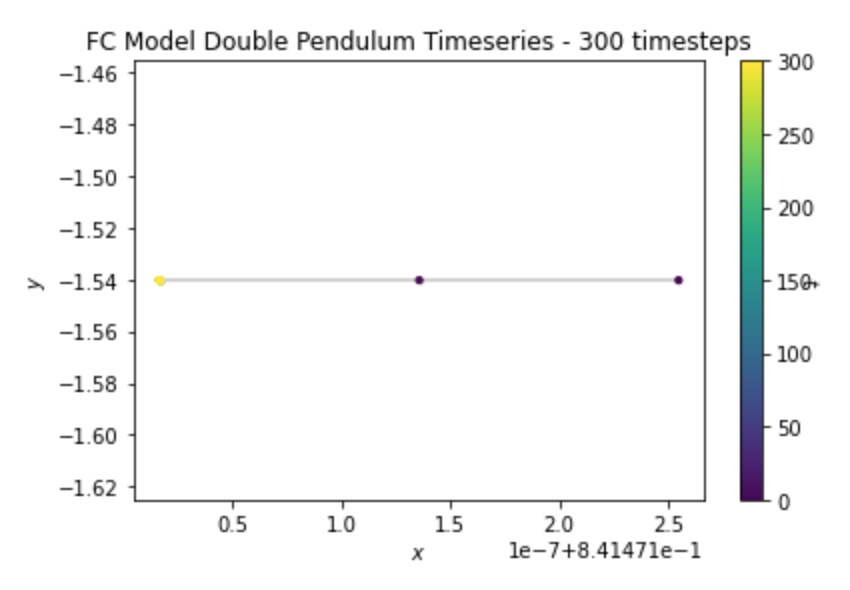
\includegraphics[width=\textwidth]{fc_pendulum.png}
			\caption{TODO Динамика системы с помощью Neural ODE}
			\label{fig:five over x}
		\end{subfigure}
		\begin{subfigure}[b]{0.49\textwidth}
			\centering
			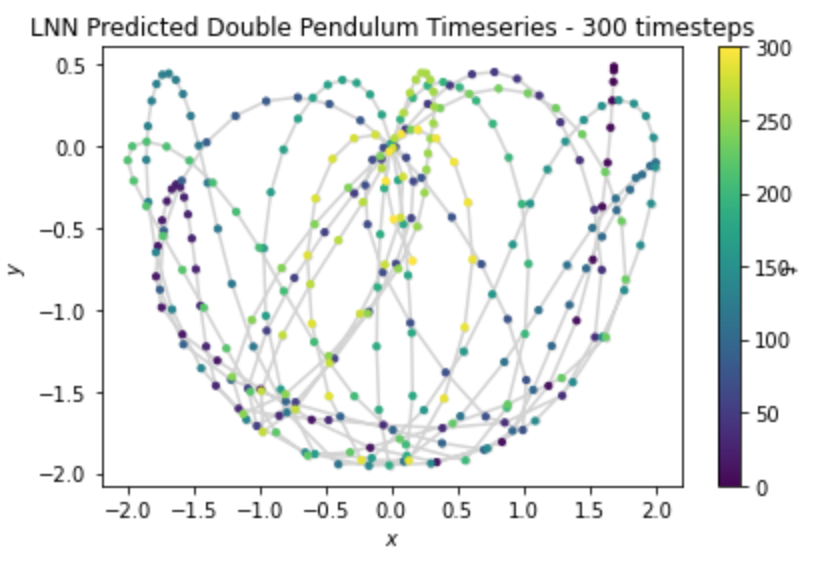
\includegraphics[width=\textwidth]{lnn_pendulum.png}
			\caption{Динамика системы с помощью LNN}
			\label{fig:five over x}
		\end{subfigure}
		\caption{Моделирование динамики системы двойного маятника различными видами нейронных сетей: аналитическое решение, полносвязная нейронная сеть, LSTM, LNN.}
		\label{fig:three graphs}
	\end{figure}
	
	
	\section{Заключение}
	В работе рассмотрена задача 
	
	\bibliographystyle{unsrt}
	\bibliography{Severilov2022MasterThesisCite.bib}

	%\bibliographystyle{unsrt}
	%\begin{thebibliography}{99}
		
	
	%	\bibitem{source_code}
%		\textit{Severilov}. Project source code is available at:~\url{https://github.com/severilov/BCI-thesis}, 2021.
	%\end{thebibliography}
	
\end{document}

